\chapter{Introduction}
\label{chap:Intro}

\section{Motivation}
\label{sec:motivation}
Software organization and developers are continuously confront the needs to
improve their software processes: the software product should meet
customers' requirements better; it should have less bugs; development
process needs to be more stable and predictable; productivity should be
improved to kick the software out of door as early as possible and so on.
Unlike other disciplines such as civil engineering and mechanic
engineering, software engineering is still too young to have mature
development process and quality control process. Software itself is very
cognitive complex because it deals with many states. Also, software
is creative and there are no two projects that
are exactly the same. Software engineering researchers and practitioners
keep generalizing and evangelizing the best practices to improve software
process.

To a software development organization there are two paths to improve its
development process: one is to find problems and solve them internally; the
other is to adopt successful practices from others. Internal software
process improvement program is called process quality control and
improvement. It is heavily emphasized by SEI's capability maturity model
(CMM). Personal Software Process (PSP) and Team Software Process (TSP) are
good examples of this category.  Adopting best practices from others is
another way to improve software process by borrowing others' successful
experiences. Usually it comes with the introduction of new technologies in
current development process. For example, another development tool can be
used because it has more elegant features and capabilities; continuous
integration can be adopted to maintain a working version and find problems
early before they sneak into the final product; software review can be
adopted to improve software quality. Internal process improvement is
gradual and steady, while adopting best practice may bring dramatic changes
to the development process.

Best practices are from prior successful experiences and they provide a set
of guidelines and recommendations to improve software development. Although
they are proved to be successful, they may or may not be appropriate in a
new organization. Managers are either persuaded by consultants or inspired
by other projects' successful experiences. The implementation of best
practices is more or less a trial-and-error approach, and the discipline of
best practice is through management and self-control of the developers.
Since best practice implementation is passive to developers, they may or
may not accept it ubiquitously. Everett Rogers modeled the adoption process
with adoption curve \cite{Potter:02}, in which there are five kinds of
adopters when a new technology is introduced: innovators, early adopters,
early majority, late majority and laggards. Although developers may accept
best practice completely, there is still the learning process to the new
technology.  Developers may have slow start at the beginning before they
understand the best practice well. Adding these factors together, there will
have a lot uncertainesses that make it hard to determine whether a best
practice is appropriate or not. The evaluation will be error-prone if the
practice itself is hard or it needs to maintain high discipline. 

One may come up with the possible solution to add more resources to ensure
that the best practices are understood and executed well by developers.
Another possible solution is to record the development process and ask
expert to review the process execution. Both solutions are very effective
and widely used by production industry to control quality and improve
productivity but it will be very costly for software organization to use
the same approach. One apparent reason is that software is unique and can
not be mass produced with assembly line. It will be very costly to invest
management and monitoring resources on software projects to have quality
control as traditional industries do. Even though it is difficult to ensure
qualita
development process to produce good software in high quality to meet the
increasing requests and dependences on software in our society.

We propose to manage and control best practice implementation automatically
using micro-process analysis technique. The automation will drastically
reduce the cost to manage and evaluate best practice implementation. We
propose to implement a software development stream analysis (SDSA)
framework to instrument development process, construct development stream,
tokenize development stream and classify software development
micro-process. Our statement is that we can effectively inspect execution
of best practice with micro-processes. We will evaluate this framework with
a best practice called Test-Driven Development, a very popular best
practice that was formalized and evangelized by Kent Beck, the pioneer of
Extreme Programming (XP). We introduce two terms with this work:
\begin{description}
\item \textit{Software Development Stream} is the collection of
  time-stamped activities occurred in software development process.
\item \textit{Micro-Process} is a group of activities that can be tokenized
  by tokenizers in the development stream. Using buffer transition as
  example, a buffer transition micro-process starts when it is a new buffer
  and ends when developer switches to another buffer or file.
\end{description}

\section{Software Development Stream and Analysis}
Software development is a complex process. In order to automate the control
and evaluation of best practice execution.  we have to solve two
problems:(1) Data collection problem, the process data must be collected
automatically and continuously;(2) Identification and evaluation problem,
best practice must have impressive characters to be identified and measured.

\subsubsection{Data Collection with Hackystat}
In the course of software development, developers interact with tools to produce
software artifacts. The data collection system will have to collect both process
data about how developers write software and metrics of the software. Process data 
are either developers' direct interactions with development tools or the 
artifacts' changes committed by development activities. The latter approach is 
more durable to most IDEs (Integrated Development Environment) because intercepting 
IDE's operations is not supported by all IDEs. The in-process and post development 
metrics can be collected by invoking metrics utilities. 

Our data collection is provided by Hackystat, an in-process unobtrusive metric
collection system. It has more than 10 sensors to collect activity, object metrics, 
unit test, build, file commits and so on. We enhanced activity sensor to include 
compilation and refactoring activities in SDSA prototype implementation. Hackystat
stores process metric data in a centralized server in XML format. Raw sensor data
is processed to deduce development activity directly or indirectly by checking
continuous metric changes. For convenience reason each activity type is processed
separately to form development sub-steam, which has homogeneous development activities. 
With this paradigm we can merge sub-streams together to generate software development
stream. Table \ref{tab:stackstream} is a small portion of the software development 
stream whilst I worked on stack example. 
\begin{table}[!h]
\centering
  \begin{tabular}{|llll|}
  \hline
    23:43:57 & TestStack.java & ADD CLASS & package org.sci \\
    23:43:57 & TestStack.java & ADD IMPORT & import junit.framework.TestCase \\
    23:43:57 & TestStack.java & MOVE CLASS & org.sci --\textgreater TestStack.java \\
    23:44:19 & TestStack.java & ADD METHOD & void testEmptyStack() \\
    23:44:38 & TestStack.java & TEST EDIT & 6sec \\
    23:44:39 & TestStack.java & COMPILE & Stack cannot be resolved \\
    23:45:07 & Stack.java     & ADD CLASS & Stack.java \\
    23:45:07 & Stack.java     & BUFFTRANS & FROM TestStack.java \\
    23:45:34 & Stack.java     & ADD METHOD & Stack() \\
    23:45:56 & Stack.java     & PRODUCTION EDIT & 18sec \\
    23:46:02 & TestStack.java & BUFFTRANS FROM & Stack.java \\
  \hline
  \end{tabular}
  \caption{Development Stream Example}\label{tab:stackstream}  
\end{table}
Stack is a data holder with operation Last-In-Last-Out(LILO). I developed it in Java
following best practice Test-Driven Development (TDD). Because test case is created 
before code implementation in TDD, I created object \textsf{\textbf{TestStack.java}} 
at the very beginning. Test case \textsf{\textbf{void testEmptyStack()}} is added right
after since it is an easy task. The compilation of this test class failed because it
tests the non-existing \textsf{\textbf{Stack.java}} object. It drives the implementation
of \textsf{\textbf{Stack}} to eliminate test failure. This typical TDD-style 
development can be easily replayed by analyzing software development stream.

\subsubsection{Best Practice Identification and Evaluation}
Development stream has rich information on software process. It's fairly easy to analyze 
a small portion of the development stream to study best practice execution, but it is
not feasible to look up the real development stream because it may have thousands' 
activities. Cook et al \cite{Cook:95} implemented a system called Balboa to discover 
and validate formal software process with finite state machine. Chris Jen et al automate 
discovery and modeling of open source project by studying web activities with email, message 
board and instant messaging etc\cite{Jesen:02}. Similarly, we can automatically discover
and evaluate best process execution in software development with software development 
stream.

Software development best practice contains a set of rules and recommendations to regulate
development process. It either defines the order of development activities or adds new
pieces to the development process. For example, incremental build is the best practice to
audit developers' edit work and build system once there are changes being made; unit test 
best practice stresses that developers should write unit tests to improve the quality of the 
program. Because best practices are empirical and repeated in software development, the software
development stream should contain many best practice iterations when it is deployed. 


 motivates us to use rule-based system
to study the execution of best practice


In our study we decide to use rule-based system to process development
stream. It is widely used in problem-solving and very effective if the
expert knowledge can be represented as if ... then ...  rules. Below is an
example from automobile problem analysis expert system \cite{Luger:01}:
\begin{verbatim}
    Rule: 
      if 
        the engine is getting gas, and 
        the engine will turn over.
      then 
        the problem is spark plug.  
\end{verbatim}
A best practice contains a set of guidelines and recommendations, which can
be translated into rules in rule-based system. We choose JESS to implement
the development stream analysis system. JESS is a rule engine for Java
platform development by Ernest Friedman-Hill in Sandia National Laboratory.
Figure \ref{fig:DataFlow} is the data flow of software development stream
analysis system.
\begin{figure}[h] 
  \centering
  \includegraphics{figs/DataFlow.eps}
  \caption{}\label{fig:DataFlow}
\end{figure} 

\begin{comment}
Similar work has ever been done to automatically discover software process
and model development process with activity data in other institutes.
Jonathan Cook and Alexander Wolf used event-data analysis to discover
formal software process IPSW7/8 automatically \cite{Cook:95} with event
data stream, which is very similiar to development stream. Chris Jesen et
al modeled and discovered the development process with developers' web
activities\cite{} on open source projects.

  First of all, best practices are presented as guideline and
  recommendation of development, which can be converted to rules easily.
  Second, rule-based system implement the very optimized Rete search
  algorithm. Third, rule-based system is very robust on the existence of
  irrelevant data. The downside of rule-based system is that it can not
  explain how the conclusions are drawn. Although best practices may state
  their guidelines vividly, presenting them with exclusive rules is very
  hard and error-prone.
\end{comment}

\section{Test-Driven Development}
Test-Driven Development (TDD), also known as Test-First Design (TFD), is an
evolutionary approach to develop software. Traditionally, software
development follows waterfall model, in which development process is
divided into stages analysis, design, coding, testing, integration and
maintenance. Before implementation, design decision is made already. 
Program is tested by quality assurance team before it is integrated into 
system. Although incremental iterative processes replaced waterfall model 
in modern software development, each iteration is still a small 
waterfall process. Test-Driven Development changed this work flow to generate
``clean code that works.''\cite{Beck:03}

In TDD, there is no big upfront design. Design decision is made in the
development process under needs by unit tests, which are translated from
requirements. It turns development upside down \cite{Pipka:03} because unit
test drives design of implementation and it is done before implementation.

Developers just write enough code to make tests pass with simplest
implementation in TDD and refactoring is needed frequently. Kent Beck, the
pioneer of Test-Driven Development, added refactor step to ``eliminate all
the duplication created in merely getting the test to work.'' Basically
there are two fundamental rules in TDD\cite{Beck:03}:

{\it
\begin{itemize}
\item Write new code only if an automated test has failed.
\item Eliminate duplication. 
\end{itemize}
}

\begin{comment}
These two simple rules generate complex individual and group behavior with
technique implication as Kent Beck addressed\cite{Beck:03}.
{\it
\begin{itemize}
\item Developers must design organically, with running code providing feedback 
      between decisions.
\item Developers must write their own tests, because you cannot wait 10 times 
      per day for someone else to write a test.
\item Development environment must provide rapid response to small changes.
\item Designs must consist of many highly cohesive, loosely coupled
  components, just to make testing easy.
\end{itemize}
}
\end{comment}

TDD is a developer-oriented process with high discipline. Developers get
quick feedback and make design decision by frequently creating and running
unit tests. In TDD, developer are constantly confronting the task to write
unit tests. It could be a very challenging work because developers are used
to the trial-and-error mindset, with which unit tests are to verify
correctness of existing code. This approach is called Test-Last Development
(TLD) contrast to TDD. Developers incline to go back to their old habits,
especially when it is time consuming to write unit test while production
code is trivial. In the situation that Extreme Programming (XP) is not
enforced, execution of Test-Driven Development will be completely up to
developers' self-control to sustain development discipline. This makes it
hard to evaluate TDD and improve TDD practice. It is important to have 
process measurement and management, otherwise, development will be unstable 
and unpredictable\cite{Florac:99}. In worst case quality of the software 
product will drop and development team will be inferior in competition.

\section{Test-Driven Development Compliance Measurement}
To measure and inspect Test-Driven Development, we use software development 
stream technique to evaluate this test-oriented development process. We define 
development stream as the sequence of activities in software development process. 
Event stream has the same meaning as development stream in this thesis. It is 
divided into episodes with the help of tokenizers. An episode is a 
micro-process or micro-iteration in the development process, which is analyzed 
based on process regulations and rules. We define this technique software 
development stream analysis (SDSA). Zorro is the implementation of SDSA. It is 
built on top of Hackystat, an in-process automatic software metric collection
system. 

\subsection{Development Stream Tokenization}
As the sequence of software development activities, development stream
reveals software process in general. In term of Test-Driven Development,
the development stream contains \textit{Test-Driven} and \textit{Refactor} 
iterations. Developer focuses on one task only in each iteration and it ends 
with test pass. This drives us to design the tokenization mechanism to divide 
entire development stream into micro-processes. Each micro-process ends with 
test pass no matter it is \textit{Test-Driven} or \textit{Refactor} iteration. 
The tool to handle this is test-pass tokenizer.

Technically test-pass tokenizer is enough to detect iterations of
Test-Driven Development. However, in team software development, developers
also deploy their work with the whole system to make sure new code will not
break it before integration. To accommodate team software development we
defined \textit{Commit} and \textit{Command} tokenizers for integration and
deployment activities. On the other side, developers may not do TDD or
occasionally step away from TDD without frequent unit test invocations. We
defined \textit{Buffer Transition} tokenizer to divide this kind of
micro-processes into smaller buffer transition micro-processes for further
analysis.

\begin{itemize}
\item \textit{Commit tokenizer} ends an episode when it encounters a bunch
  of file commit activities. It can be used to inspect what developers do
  before integration.
\item \textit{Command tokenizer} ends an episode when there are some
  consecutive command build activities to deploy system in local
  environment.
\item \textit{Test Pass tokenizer} ends an episode when there are
  successful unit test invocations. We implemented it to find the iterations
  in Test-Driven Development.
\item \textit{Buffer Transition tokenizer} starts an episode when it
  encounters consecutive buffer transition activities. It sums what
  developers did to the working buffer.
\end{itemize}

In Zorro we chain these tokenizers together to apply them on development
stream to systematically tokenize it into micro-processes.

\subsection{Micro-process Classification and TDD Compliance}
Micro-process is also called episode in this thesis. Generally an episode
contains development activities to implement a certain functionality. In my
thesis I will classify the episode on micro-process level to study
compliance of Test-Driven Development. Rule-engine is a natural choice for
this task because it can find the skeleton of development structure in the
existence of noise. Test-Driven Development implies the order of
development is to ``test a little, code a little and repeat."\cite{Beck:03}
The episode that follows this order is \textit{Test-First}, otherwise it
will be \textit{Test-Last}. An episode is \textit{Refactor} if there is no
new test case creation but code implementation and unit test invocations.
Rich rules are defined to classify micro-process to study TDD in Zorro.

\section{Thesis Structure}
In my thesis work I implemented Zorro to study software development and
Test-Driven Development in specific. It looks at software development in
fine-grained details. Chapter \ref{chap:RelatedWork} is the literature
review. It is mainly about personal software process, extreme programming
(XP), unit testing and process conformance studies. Chapter
\ref{chap:Implementation} explains implementation of Zorro and it is
evaluated in chapter \ref{chap:Evaluation}.  The conclusion and discussion
will come out after case studies.

\begin{comment}

 as in Figure \ref{fig:EpisodeTree}.

\begin{figure}[htbp] 
  \centering
  \includegraphics[width=0.8\textwidth]{figs/EpisodeTree.eps}
  \caption{Episode Tree}\label{fig:EpisodeTree}
\end{figure} 


Some empirical case studies \cite{George:03}, \cite{Maximilien:03}
reported successes on TDD practice. According to these studies TDD group
passed more black box tests than TLD group and they spent less time on
projects than TLD group. Even though most empirical studies drew positive
conclusion on Test-Driven Development there are still some neutral or
negative reports on TDD. Geras etc. \cite{Geras:04} found that there is
little or no difference in developer productivity in TDD and TLD processes.
Another study \cite{Muller:02} concluded that TDD does not accelerate the
implementation and the resulting programs are not more reliable than TLD.

\section{Validation}
Unlike many other cumbersome software processes such as Spiral model, PSP or
RUP Test-Driven Development is very lightweight. It contains two simple
rules only. In practice TDD is hard to follow compared to other processes
because there is no management involved in the development. In situations
that pair programming is not involved developers are fully responsible for
TDD execution by themselves without monitoring. This weakness will bring
many questions to TDD process. Do developers do Test-Driven Development
when they are told to do so? And if they do how well they do TDD in their
development? Do developers always follow two TDD rules?

In my thesis study I will build a system on top of Hackystat to answer
these questions as well as provide a tool to discipline TDD process.  There
are two goals to pursue in my work. One is to study how the development is
being done, especially how the unit testing is conducted in Test-Driven
Development. Another goal is to study properties of TDD. Will developers
spend more time on development and yield high quality code or not? Will the
test coverage be naturally 100\%?

Scott Ambler's UML diagram (Figure \ref{fig:TDDSteps}) depicts TDD development
iterations.

\begin{figure}[htbp] 
  \centering
  \includegraphics{figs/TDDSteps.eps}
  \caption{The Steps of TDD}\label{fig:TDDSteps}
\end{figure} 

\begin{itemize}
\item The first step is to add a test quickly. Basically it just fails the
  code.
\item Next run your test or test suite to make sure the new test does fail.
\item Make changes to the function code to make test pass. As long as it
  can make test pass you even can fake the implementation, for instance,
  return a constant number.
\item Run your tests again. If it still fails you go ahead to update your
  function code. Once all tests pass you can start over with a new test.
\end{itemize}



 
In the early era of software development there is no software process.
Software systems are developed in a chaotic style and their successes
depended largely on individual's skills and capabilities. Water-fall model
is the first and most popular software development process and it still
exists in many organizations. In water-fall model software development is
divided into stages from requirement analysis to operation and testing is
conducted after project is implemented. Bugs and defects found in testing
will be fed back to the development team or maintenance team. Since bugs
and defects are revealed at the late stage of software development
water-fall model is reluctant to meet customer's requirements and defect
fix. If defects are rooted from design it will be extremely hard to adapt
changes according to water-fall model.

Modern iterative incremental development(IID) was developed to fix this
problem by dividing a large project into many parts.  They are implemented
iteratively. Each iteration can be a mini-waterfall process so that defects
can be fixed and changes can be made very quickly.  Spiral model is the
first process definition to formulate iterative incremental development
practice. Other variations like prototyping, RAD, CleanRoom, Scrum, RUP,
FDD, Extreme Programming are used in many projects successfully.  Latest
development of continuous integration builds system once a day. In these
processes testing is done after some amount of work is finished to improve
project quality.
  
\section{Personal Software Process}
\label{sec:psp}

   Introduce LEAP and Hackystat.

\section{Test-Driven Development}
\label{sec:tdd}

\subsection{Unit Testing}
\label{sec:UnitTest}
Object-oriented technique treats abstract concepts as entities such that
each of them is independent and can exist without relying on other code.
Unit testing was invented to test a component before it is integrated to
interact with other components. Unit testing originates from
pre-object-oriented era and an individual test concentrates on a single
unit of the system rather than on the entire system. At present when we say
unit testing it refers to component testing. In object-oriented world a
component test usually tests an object or class which is the smallest component
of a system. ``In computer programming, a unit test is a method of testing the
correctness of a particular module of source code.'' \cite{UnitTestWiki}

Unit testing is becoming more and more popular in modern software
development.  The de facto unit testing standard, ``xUnit'' framework, is
already ported to more than 30 language support. It makes test automation
be feasible and test cases created with XUnit framework can server as
regression test suite too. Except for verifying correctness of each class
unit testing is also the executing documentation. In recent software
project development unit testing is integrated into development process in
many organizations. Test cases are written by developers who are also
responsible for programs. Even though source code is visible to developers
but unit testing is still thought as black-box testing because it simulates
calls from other components.  

JUnit is the most well-known XUnit framework implementation in software
development and other dialects NUnit, CPPUnit, PyUnit so on and so forth
are created to make writing unit tests be very simple in different
programming languages. JUnit and NUnit also have IDE plug-in supports so
that a unit test case can be exercised by just a single click. For
continuous integration unit test cases can also be batched together to run
as ANT task. Since writing unit tests is not a cumbersome job any more it
is recommended to write unit tests in the development process instead of
allocating extra resource to let quality assurance testers to create unit
tests separately. It improves the effectiveness of testing such that
software systems are in high quality before they are delivered to quality
assurance department or customers if there is no quality assurance process.
Since less time is needed to do quality assurance it will save overall
development time conceptually.


In TDD unit testing is crucial because it drives the implementation and provides
instant feedback of the developing code to the developers. The XUnit
framework family make it easy to write tests and execute tests often in
software development.

\section{Thesis Work}


\section{Road Map}

\end{comment}
\begin{comment}
\label{sec:ResearchObjective}
Test-Driven Development is being accepted by more and more developers and
organizations. On the other side there are still many developers and
researchers resist Test-Driven Development or doubt its effectiveness in
software development. Kent Beck argued that TDD will not increase
development cost but can actually improve productivity as well as software
quality. Ron Jeffries's pithy word ``Clean code that works'' is the goal
of Test-Driven Development.


\section{Extreme Programming(XP) and Test-Driven Development(TDD)}
[How good is unit test? and why TDD]

  
This testing pyramid corresponds to software system development process.
In general a large system is divided into many components to be implemented
independently. Unit testing is created to verify correctness of each
component before it is integrated into the system.
  
Usually unit testing is done by programmers themselves to verify the
correctness or by quality assurance specialists to find errors in the
existing code.  According to the cost model of removing bugs in different
software development stages removing bugs in development phase is the most
cost-effective way.  Because unit testing is good from many aspects Extreme
Programming, an agile software development process, advocates Test-Driven
Development (TDD) as its core component. In TDD unit tests are
incrementally written prior to code implementation \cite{George:03} thus
it drives software specification design in addition to validating and
verifying program correctness. Because of this capability TDD is also
called Test-First Design (TFD). As comparison the old way writing unit
tests after code is ready is called Test-Last Development(TLD).
  
  Some empirical case studies \cite{George:03}, \cite{Maximilien:03}
  reported successes on TDD practice. According to these studies TDD group
  passed more black box tests than TLD group and they spent less time on
  projects than TLD group. Even though most empirical studies drew positive
  conclusion on Test-Driven Development there are still some neutral or
  negative reports on TDD. Geras etc. \cite{Geras:04} found that there is
  little or no difference in developer productivity in TDD and TLD
  processes. Another study \cite{Muller:02} concluded that TDD does not
  accelerate the implementation and the resulting programs are not more
  reliable than TLD.
  
  The controversial conclusions can be either from TDD process itself or
  from the poorly executed experiments. There is one thing in common that
  all these studies failed to address how they managed experiments to
  guarantee TDD developers do Test-Driven Development while TLD developers
  do Test-Last Development in their studies. There is no process data
  available to crossly validate process disciplines. The lack of
  fine-grained process data and software metrics makes it impossible to
  conclude whether developers were doing TFD, ad-hoc or TLD in the previous
  experiments; thus, conclusions drawn from these experiments are weakened
  and become questionable. In my thesis I will add in-process metric
  support provided by Hackystat to study how unit tests are created and
  exercised in the development process to regulate software development.
\end{comment}

\begin{comment}  
\section{Testing}
\label{sec:Testing}
Testing is very important to software project success because developers
can not always produce perfect code that works well at the first time. Many
reasons determine that we need testing in software development. First of
all, many software systems deal with large number of states with complex
algorithms, also it is hard and impossible to address all system
requirements at the beginning of software projects development. Developers
always have to deal with new and changing requirements during the
development.  Another important factor is that software projects are
written by developers.  As human beings developers are not good at
repeative programming work without committing mistakes.  Since software
development is error-prone many design and development support tools such
as flowchart, dash board, UML , compilers, debuggers, version control
system, project management software, bug tracking system and software
review etc are brought up to support qualitative software development.
Moreover, there are rare software projects developed and maintained by an
individual programmer nowadays. The ineffective collaboration and
cooperation in the developing team will make software volatile to defects
and bugs too \cite{Pfleeger:01}.  To ensure software quality there are
quality assurance departments in many software institutes and many testing
techniques appeared in the development of software engineering discipline.
From visibility of source code there are white-box testing and black-box
testing. Depending on when testing happens there are unit testing,
regression testing, integration testing, system testing and acceptance
testing which can be done by programmers, quality assurance testers or
customers manually or automatically.

\begin{figure}[ht] 
  \centering
  \includegraphics[width=0.5\textwidth]{figs/TestLayerPyramid.eps}
  \caption{Software Testing Pyramid}\label{fig:TestLayer}
\end{figure} 

In tradition, software testing is thought as quality assurance testers' or
customers' job in water-fall software process model. Even in recent
iterative incremental development (IID) models quality assurance
specialties and customers still play important roles on testing.


\section{Software Processes}
\label{sec:SoftwareProcess}
In the early era of software development there is no software process.
Software systems are developed in a chaotic style and their successes
depended largely on individual's skills and capabilities. Water-fall model
is the first and most popular software development process and it still
exists in many organizations. In water-fall model software development is
divided into stages from requirement analysis to operation and testing is
conducted after project is implemented. Bugs and defects found in testing
will be fed back to the development team or maintenance team. Since bugs
and defects are revealed at the late stage of software development
water-fall model is reluctant to meet customer's requirements and defect
fix. If defects are rooted from design it will be extremely hard to adapt
changes according to water-fall model.

Modern iterative incremental development(IID) was developed to fix this
problem by dividing a large project into many parts.  They are implemented
iteratively. Each iteration can be a mini-waterfall process so that defects
can be fixed and changes can be made very quickly.  Spiral model is the
first process definition to formulate iterative incremental development
practice. Other variations like prototyping, RAD, CleanRoom, Scrum, RUP,
FDD, Extreme Programming are used in many projects successfully.  Latest
development of continuous integration builds system once a day. In these
processes testing is done after some amount of work is finished to improve
project quality.



\section{Extreme Programming}
\label{sec:XP}
Extreme programming (XP) grows very fast recently and many organizations
are using it or considering to adopt it in their developments. Extreme
Programming is also one kind of iterative incremental development (IID)
process.  It begins with collecting ``user stories'', which are brief
description of tasks to be accomplished. Developers can discuss with on-site
customers to make release plan based on user stories. After each release
customer can test the sub system and give feedback to developers quickly.
XP can not only meet customers' changing requirements well but also provide
high quality code because it stresses heavily on unit tests in the
development. Four rules are enforced in extreme programming.

\begin{itemize}
\item All code must have unit tests.
\item All code must pass all unit tests before it can be released.
\item When a bug is found tests are created.
\item Acceptance tests are run often and the score is published.
\end{itemize}

To enact these rules XP projects should be developed in Test-Driven
Development process, in which unit tests are created before code
implementation.  Developers write unit tests based on user stories first
and then generate code to make test pass.
\end{comment}
